% !TEX root = ../slides.tex

\begin{frame}[label=coeff_in_zero]
\frametitle{Walsh coefficients $\widehat{F}(0, \beta)$}
\vspace{-10pt}

\onslide<+->{
\recapbox{\emph{Subspace prop}: $\forall \ \clambda, \quad \cF(\clambda\cFF) = \cF(\clambda)\cFF$. \hfill $ \cF(\clambda\cphi) = \cF(\clambda)\cGl(\cphi)$, with $\cGl \from \cFF \xrightarrow{\sim} \cFF$\vspace{5pt}

\hspace*{15pt} $\cFh(\alpha, \beta) \vcentcolon= \sum\limits_{\clambda \in \cLL} (-1)^{\alpha\cdot\clambda + \beta\cdot F(\clambda)}$
\hspace*{15pt} $N_{\clambda} \vcentcolon= \frac{\card{F^{-1}(\clambda\cFF)}}{\card{\cFF}}$}
}

\onslide<+->{
\begin{mybox}[cred]{Walsh coefficients in zero}
$\cF$ satisfying the subspace property. $[\cLL : \cFF] = 2$. Then
$$ \forall \ \beta \in \cLL^*, \quad \cFh(0, \beta) = 2^{t}(N_{\beta^{-1}} - 1)\vspace{10pt}$$

% Proof: $ \cFh_\beta(0) = -2^t + \sum_{\cgamma \in \cGamma} \cGhl\left(0, \trlf\left(\beta F(\cgamma)\right)\right) = -2^t +  \sum_{\cgamma \in \cGamma} 2^t\delta_{0, \trlf(\beta F(\cgamma))}$

% \vspace{6pt}
% $\trlf = X + X^{t}$, so $\ker(\trlf) = \cFF$.
\end{mybox}}

\only<3>{
\centering
\large Kim mapping \vspace{5pt}


\includegraphics[scale=.22]{figures/kim_lat_first_row}

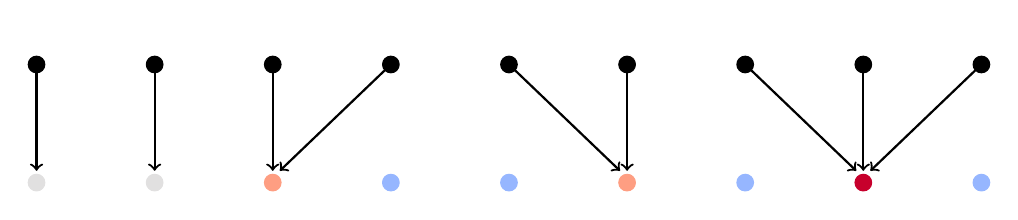
\begin{tikzpicture}[scale=.3]

\definecolor{orangeLAT}{HTML}{fe9e82}
\definecolor{redLAT}{HTML}{c7002c}
\definecolor{lightblueLAT}{HTML}{96b6ff}
\definecolor{blueLAT}{HTML}{4851cc}
\definecolor{greyLAT}{HTML}{e1e0e0}

\foreach \x in {0,1,...,8} {
 \draw[black, fill = black] (\x*5,0) circle (10pt);
}

\draw[thick, ->] (0,0) -- (0, -4.5);
\draw[thick, ->] (5,0) -- (5, -4.5);
\draw[thick, ->] (10,0) -- (10, -4.5);
\draw[thick, ->] (15,0) -- (10.3, -4.5);
\draw[thick, ->] (20,0) -- (24.7, -4.5);
\draw[thick, ->] (25,0) -- (25, -4.5);
\draw[thick, ->] (30,0) -- (34.7, -4.5);
\draw[thick, ->] (35,0) -- (35, -4.5);
\draw[thick, ->] (40,0) -- (35.3, -4.5);


\draw[greyLAT, fill = greyLAT] (0,-5) circle (10pt);
\draw[greyLAT, fill = greyLAT] (5,-5) circle (10pt);
\draw[orangeLAT, fill = orangeLAT] (10,-5) circle (10pt);
\draw[lightblueLAT, fill = lightblueLAT] (15,-5) circle (10pt);
\draw[lightblueLAT, fill = lightblueLAT] (20,-5) circle (10pt);
\draw[orangeLAT, fill = orangeLAT] (25,-5) circle (10pt);
\draw[lightblueLAT, fill = lightblueLAT] (30,-5) circle (10pt);
\draw[redLAT, fill = redLAT] (35,-5) circle (10pt);
\draw[lightblueLAT, fill = lightblueLAT] (40,-5) circle (10pt);

\draw[transparent] (0, 1.5) circle (1pt);
\end{tikzpicture}
}

\only<4>{
\centering
\large Cube\vspace{5pt}


\includegraphics[scale=.22]{figures/cube_lat_first_row}
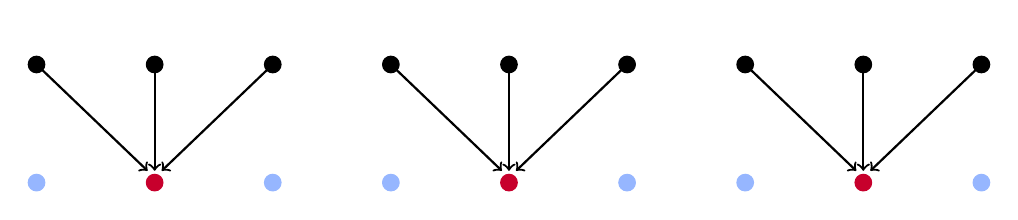
\begin{tikzpicture}[scale=.3]

\definecolor{orangeLAT}{HTML}{fe9e82}
\definecolor{redLAT}{HTML}{c7002c}
\definecolor{lightblueLAT}{HTML}{96b6ff}
\definecolor{blueLAT}{HTML}{4851cc}
\definecolor{greyLAT}{HTML}{e1e0e0}

\foreach \x in {0,1,...,8} {
 \draw[black, fill = black] (\x*5,0) circle (10pt);
}

\draw[thick, ->] (0,0) -- (4.7, -4.5);
\draw[thick, ->] (5,0) -- (5, -4.5);
\draw[thick, ->] (10,0) -- (5.3, -4.5);
\draw[thick, ->] (15,0) -- (19.7, -4.5);
\draw[thick, ->] (20,0) -- (20, -4.5);
\draw[thick, ->] (25,0) -- (20.3, -4.5);
\draw[thick, ->] (30,0) -- (34.7, -4.5);
\draw[thick, ->] (35,0) -- (35, -4.5);
\draw[thick, ->] (40,0) -- (35.3, -4.5);


\draw[lightblueLAT, fill = lightblueLAT] (0,-5) circle (10pt);
\draw[redLAT, fill = redLAT] (5,-5) circle (10pt);
\draw[lightblueLAT, fill = lightblueLAT] (10,-5) circle (10pt);
\draw[lightblueLAT, fill = lightblueLAT] (15,-5) circle (10pt);
\draw[redLAT, fill = redLAT] (20,-5) circle (10pt);
\draw[lightblueLAT, fill = lightblueLAT] (25,-5) circle (10pt);
\draw[lightblueLAT, fill = lightblueLAT] (30,-5) circle (10pt);
\draw[redLAT, fill = redLAT] (35,-5) circle (10pt);
\draw[lightblueLAT, fill = lightblueLAT] (40,-5) circle (10pt);

\draw[transparent] (0, 1.5) circle (1pt);
\end{tikzpicture}
}


\end{frame}